%\documentclass[12pt]{article}  % standard LaTeX, 12 point type
\documentclass{sig-alternate}
%\usepackage{amsfonts,latexsym}
%\usepackage{amsthm}
%\usepackage{amssymb}
\usepackage[utf8]{inputenc} % Кодировка
\usepackage[english]{babel} % Многоязычность
%\usepackage{algpseudocode}
%\usepackage{algorithm}
%usepackage{algorithmicx}
%\usepackage{amsmath}

%\usepackage{color}
%\usepackage{listings}
\usepackage{caption}
\usepackage{graphicx}
%\usepackage{ucs}

\graphicspath{{pics/}}



\begin{document}

\makeatletter
\def\@copyrightspace{\relax}
\makeatother

\title{From grammar to shared packed parse forest}

\sloppy

\numberofauthors{1}

\author{
\alignauthor
       Semyon Grigorev\\
       \affaddr{Saint Petersburg State University}\\
       \affaddr{7/9 Universitetskaya nab.}\\
       \affaddr{St. Petersburg, 199034 Russia}\\
       \email{semen.grigorev@jetbrains.com}
}

\maketitle

It is possible to build graph structured representation of result which can be interesting for several reasons.
\begin{itemize}
\item More user friendly query result represenation. 
\item Useful for query result explorationa and investigation.
\item Useful for query debugging.
\end{itemize}

Example from your article~\cite{jelle} will be used for explanation. Let we intrioduce new notation for nonterminals and terminals for simplification.

\begin{align*}
q_1 = q[A,B] \quad & q_5 = q[C,E] \\
q_2 = q[A,C] \quad & q_6 = q[A,D] \\
q_3 = q[D,E] \quad & q_7 = q[A,E] \\
q_4 = q[B,D] \quad & q_8 = q[B,E] 
\end{align*}

\begin{align*}
T_1 = friendOf_{A,B} \quad & T_4 = friendOf_{B,D}\\
T_2 = friendOf_{A,C} \quad & T_5 = friendOf_{C,E} \\
T_3 = friendOf_{D,E} \quad &  \\
\end{align*}

Now grammar from~\cite{jelle}(pages 6-7) can be represented as below. Let it be named $G_1$

\begin{align*}
q_1 \rightarrow T_1 \quad & q_6 \rightarrow q_1 \ q_4  \\
q_2 \rightarrow T_2 \quad & q_7 \rightarrow q_2 \ q_5  \\
q_3 \rightarrow T_3 \quad & q_7 \rightarrow q_1 \ q_8  \\
q_4 \rightarrow T_4 \quad & q_7 \rightarrow q_6 \ q_3  \\
                    \quad & q_8 \rightarrow q_4 \ q_3  \\
\end{align*}


For each context-free grammar we can create regular tree grammar~\cite{tata}(section 2.4). Moreover if $G$ is a context-free word grammar, then the set of derivation trees of
$L(G)$ is a regular tree language. By using algorithm presented in~\cite{tata}(section 2.4) we can build regular tree grammar $G_2$ for grammar $G_1$:

\begin{align*}
q_1 \rightarrow q_1(T_1) \quad & q_6 \rightarrow q_6(q_1, q_4)  \\
q_2 \rightarrow q_2(T_2) \quad & q_7 \rightarrow q_7(q_2, q_5)  \\
q_3 \rightarrow q_3(T_3) \quad & q_7 \rightarrow q_7(q_1, q_8)  \\
q_4 \rightarrow q_4(T_4) \quad & q_7 \rightarrow q_7(q_6, q_3)  \\
                         \quad & q_8 \rightarrow q_8(q_4, q_3)  \\
\end{align*}


Reduced graph. It is SPPF.

\begin{figure}[h]
    \begin{center}
        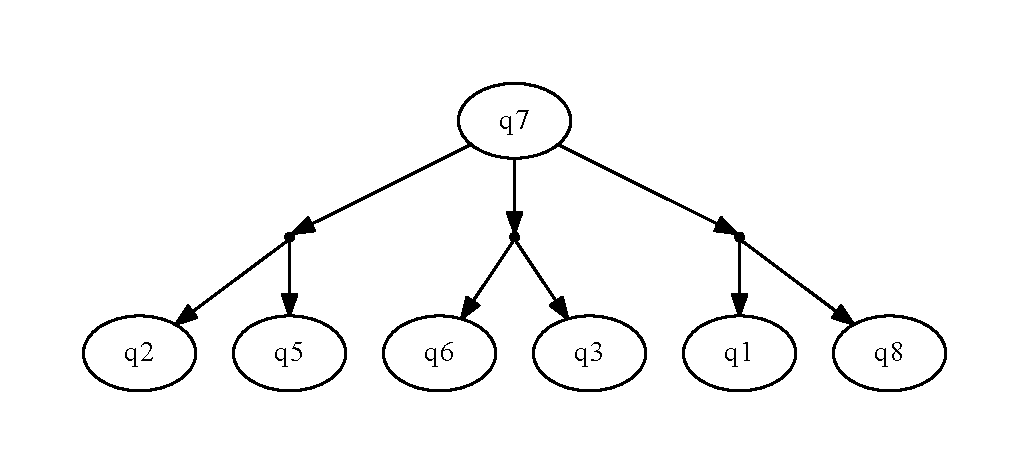
\includegraphics[width=6cm]{altsInSPPF.pdf}
        \caption{Input graph $M$}
        \label{input}        
    \end{center}
\end{figure}


\begin{figure}[h]
    \begin{center}
        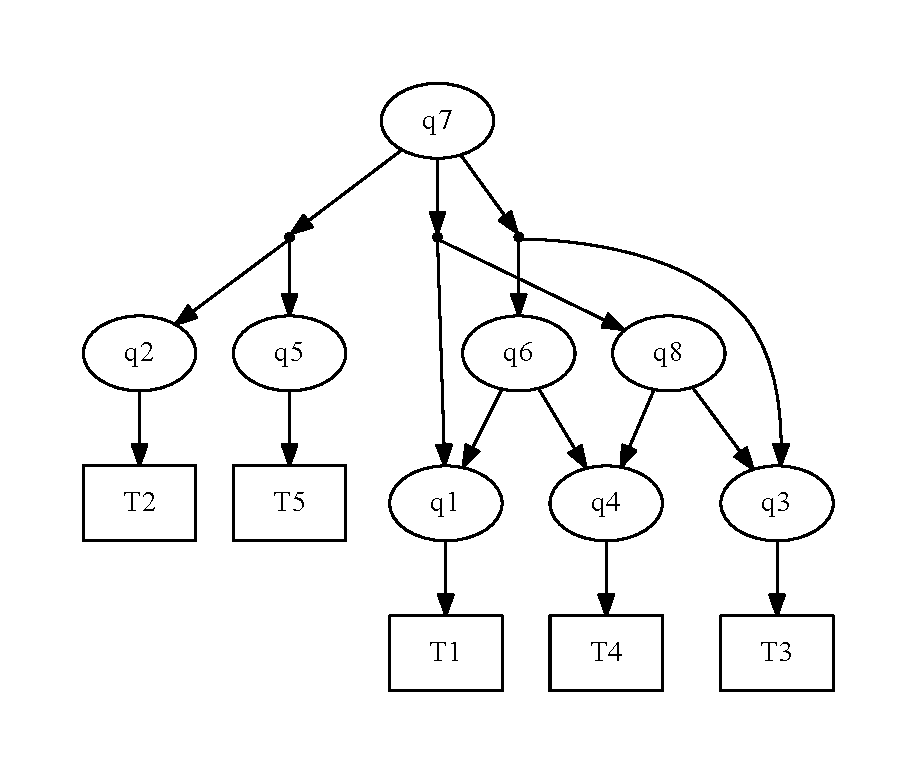
\includegraphics[width=6cm]{cleanSPPF.pdf}
        \caption{Input graph $M$}
        \label{input}        
    \end{center}
\end{figure}


Let return information about edges back.


\begin{figure}[h]
    \begin{center}
        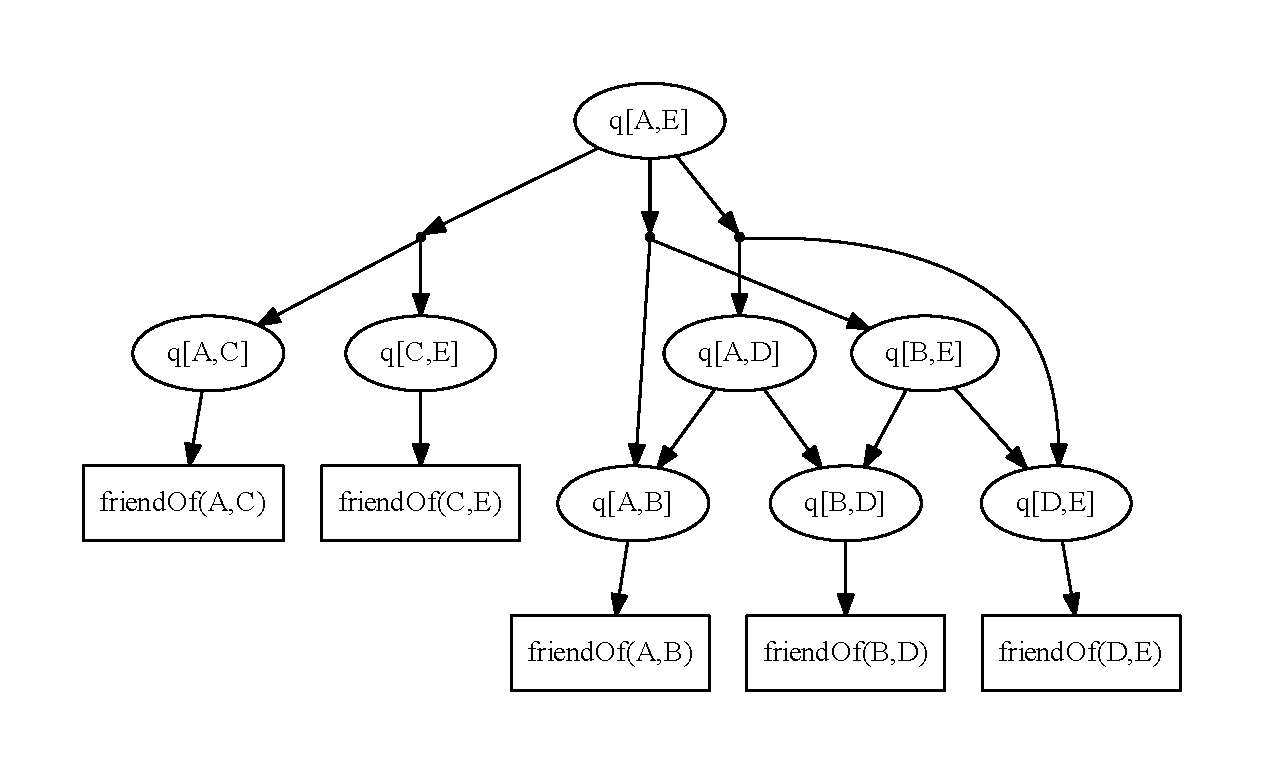
\includegraphics[width=8cm]{resultSPPF1.pdf}
        \caption{SPPF with information about paths}
        \label{SPPF2}        
    \end{center}
\end{figure}


It is possible to build SPPF with our tool without to CNF transformation.

Query grammar.
\begin{figure}[h]
   \begin{center}
\begin{verbatim}
   0: s = L s R 
   1: s = middle
   2: middle = L R
\end{verbatim}
   \caption{Grammar $G_1$ for language $L=\{L^n R^n; n \geq 1\}$}
   \label{grammarG}        
   \end{center}
\end{figure}


Input graph.

\begin{figure}[h]
    \begin{center}
        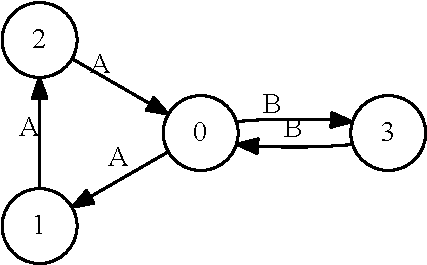
\includegraphics[width=6cm]{input.pdf}
        \caption{SPPF with information about paths}
        \label{SPPF2}        
    \end{center}
\end{figure}

Query result

\begin{figure}[h]
    \begin{center}
        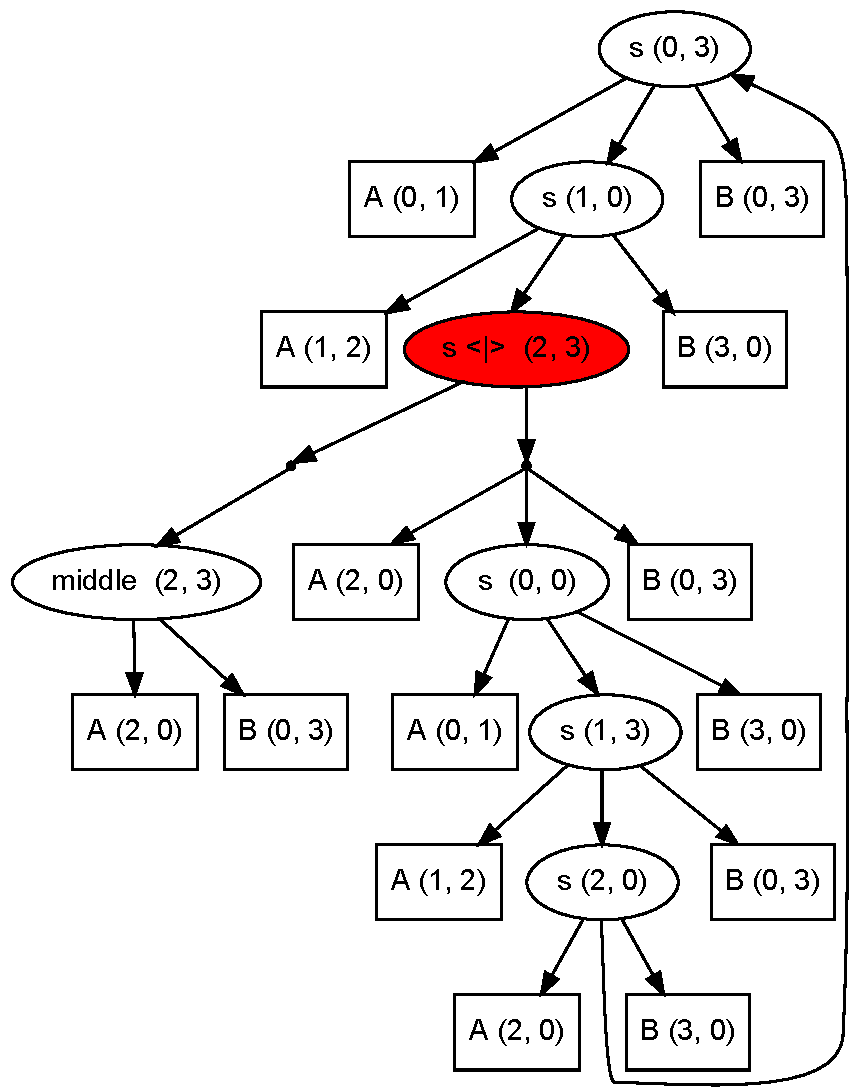
\includegraphics[width=8cm]{AnBn.pdf}
        \caption{SPPF with information about paths}
        \label{SPPF2}        
    \end{center}
\end{figure}



\begin{thebibliography}{9}

\bibitem{tata}
  Comon, Hubert, et al. "Tree automata techniques and applications." (2007).

\bibitem{jelle}
Hellings, Jelle. "Querying for Paths in Graphs using Context-Free Path Queries." arXiv preprint arXiv:1502.02242 (2015).

\end{thebibliography}


\end{document}